\documentclass[7pt]{article}

\usepackage{amsmath}
\usepackage{graphicx}
\usepackage{caption}
\usepackage[landscape]{geometry}
\usepackage{multicol}
\usepackage{amssymb}

\usepackage{geometry}
\geometry{
 a4paper,
 total={285mm,185mm},
 left=10mm,
 top=10mm,
}

\setcounter{section}{2}
\setlength\columnseprule{0.5pt}
\setlength{\parindent}{0pt}
\graphicspath{ {images/} }

\begin{document}
\begin{multicols*}{3}

\section{Dynamik}

\subsection{Definitionen}

\subsubsection{Masse}

Masse ist Eigenschaft eines K{\"o}pers $\Rightarrow$ {\"u}berall gleich (im Gegensatz zu Gewicht).

\subsubsection{Lineare Impuls}

Der lineare Impuls ist definiert als
\begin{equation*}
	p = mv \qquad\text{mit Einheit}\qquad \frac{kg\cdot m}{s}
\end{equation*}

\begin{equation*}
	\frac{m_A}{m_B} = \frac{v_B}{v_A} \Rightarrow p_A + p_B = 0
\end{equation*}

In einem isolierten System ist der \textbf{Gesamtimpuls} erhalten.

\subsubsection{Kraft}

Die Kraft ist die zeitliche {\"a}nderung des Impulses:
\begin{equation*}
	F = ma(t) \qquad\text{mit Einheiten}\qquad 1N = \frac{kg\cdot m}{s^2}
\end{equation*}

\subsection{Newtonsche Gesetze}

\subsubsection{Tr{\"a}gheitsprinzip}

Ein K{\"o}per bleibt in Ruhe oder bewegt sich mit konstanter Geschwindigkeit, wenn er isoliert ist.

\subsubsection{Aktionsprinzip}

Die Beschleunigung eines K{\"o}pers ist umgekehrt proportional zu seiner Masse und direkt proportional zur resultierenden Kraft, die auf ihn wirkt. 

\subsubsection{Aktions-Reaktions-Prinzip}

Zu jeder Aktion geh{\"o}rt eine gleich grosse Reaktion, die denselben Betrag besitzt aber in die entgegengesetzte Richtung zeigt.

\subsection{Raketenantrieb}

\begin{enumerate}
	\item [$v(t)$] Geschwindigkeit der Rakete bez{\"u}glich dem festen Koordinatensystem
	\item [$u$] Konstante Ausstossgeschwindigkeit des Gases \emph{relativ zur Rakete} (relativ zum festgelegten Koordinatensystem mit Geschwindigkeit $v-u$)
	\item [$M(t)$] Gesamtmasse, also Rakete + Treibstoff zur Zeit $t$
\end{enumerate}

Der \textbf{Gesamtimpuls} der Rakete zur Zeit $t$ ist gleich
\begin{equation*}
	p(t) = M(t)v(t)
\end{equation*}

Auf die Rakete wirkt die \textbf{Schubkraft $F$}
\begin{equation*}
	F = u\frac{dm}{dt}
\end{equation*}

Und die \textbf{Geschwindigkeit}
\begin{equation*}
	v(t) - v_0 = -u(\ln(M_0 - m) - \ln(M_0))\\
\end{equation*}
wobei $M_0$ die Anfangsmasse und $m$ die Gesamtmasse des ausgestossenen Gases ist. \newline
Oder als Funktion der ausgestossenen Masse (mit $v_0 = 0$)
\begin{equation*}
	v = u\ln(\frac{1}{1-\frac{m}{M_0}})
\end{equation*}

\subsection{Schiefe Ebene}

\subsubsection{Statischer Fall}

\begin{center}
	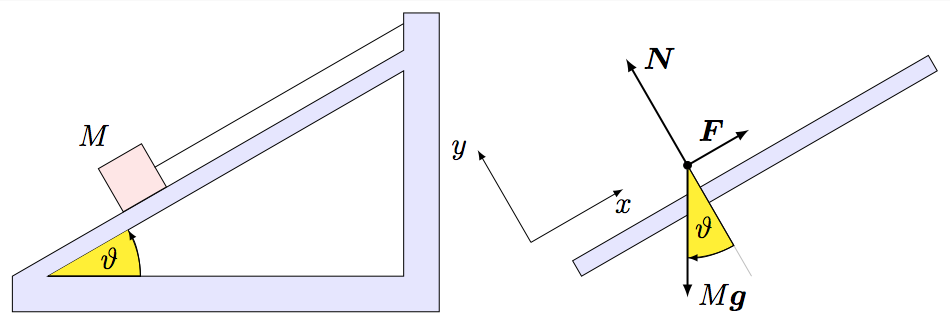
\includegraphics[width=200pt]{images/schiefe_ebene}
\end{center}

\begin{equation*}
	F + N + Mg = 0\\
\end{equation*}

Daraus folgt
\begin{equation*}
\begin{split}
	F & = Mg\sin(\vartheta)\\
	N & = Mg\cos(\vartheta)
\end{split}
\end{equation*}

\subsubsection{Dynamischer Fall}

\begin{equation*}
	N + Mg = F_{res} = Ma
\end{equation*}

Dank der Normalkraft verschwindet die Beschleunigung in $y$-Richtung.
In $x$-Richtung ist sie gleich
\begin{equation*}
	a_x = -g\sin(\vartheta)
\end{equation*}

\subsection{Federkraft}

\begin{equation*}
	F = -k(x-x_0) = -k\Delta x
\end{equation*}

wobei $k$ die Federkonstante mit Einheit $\frac{N}{m}$, $x_0$ die L{\"a}nge der Feder im unbelasteten Zustand ist.

\subsection{Bewegung mit Rollen}

\begin{center}
	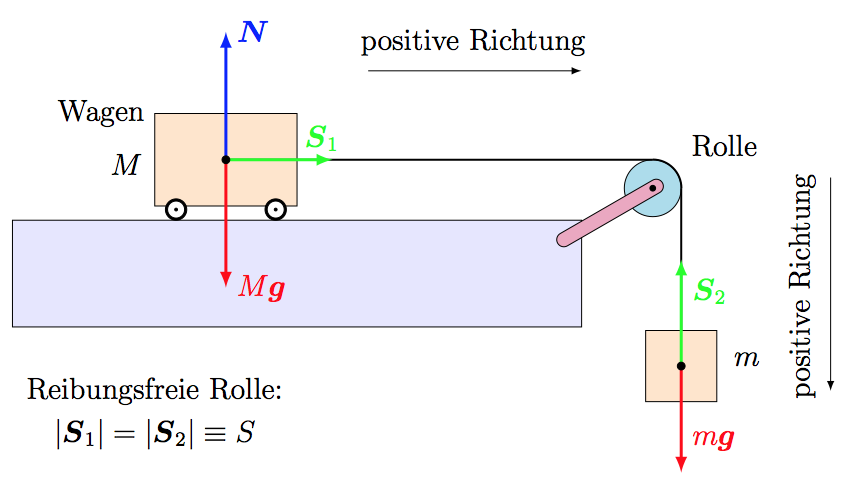
\includegraphics[width=200pt]{images/bewegung_rollen}
\end{center}

\begin{equation*}
\begin{split}
	S & = Ma \\
	a & = \frac{m}{M + m}g
\end{split}
\end{equation*}

\subsection{Atwoodsche Fallmaschine}

\begin{center}
	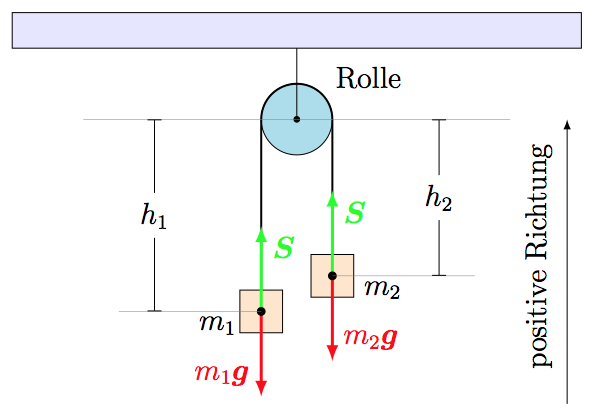
\includegraphics[width=200pt]{images/fallmaschine}
\end{center}

\begin{equation*}
\begin{split}
	a_1 & = -a_2 = \frac{m_2-m_1}{m_2+m_1}g \\
	  S & = \frac{2m_1m_2}{m_1+m_2}g \qquad\text{wobei}\qquad |a_1|=|a_2| < g
\end{split}
\end{equation*}

\subsection{Harmonische Schwingungen}

\begin{equation*}
\begin{split}
	x(t) & = A\sin(\omega t+\delta)\\
	v(t) & = A\omega\cos(\omega t + \delta)\\
	a(t) & = -A\omega^2\sin(\omega t+\delta) = -\omega^2x(t)
\end{split}
\end{equation*}
wobei $A$ die Amplitude, $\omega$ die Kreisfrequenz und $\delta$ die Phasenkonstante ist.
\newline

Die \textbf{Kreisfrequenz $\omega$} h{\"a}ngt dabei nur von der R{\"u}ckstellkraftkonstante $k$ und der Masse $m$ ab
\begin{equation*}
	\omega = \sqrt{\frac{k}{m}}
\end{equation*}

Der Winkel der Sinusfunktion wird als \textbf{Phase} der Schwingung bezeichnet
\begin{equation*}
	\varphi(t) = \omega t + \delta
\end{equation*}
wobei $\delta$ die urspr{\"u}ngliche Phase zur Zeit $t = 0$ ist. \newline

Die \textbf{Periode $T$} ist die Zeit, die ben{\"o}tigt wird, um eine vollst{\"a}ndige Schwingung durchzuf{\"u}hren
\begin{equation*}
	T = \frac{2\pi}{\omega} = 2\pi\sqrt{\frac{m}{k}}
\end{equation*} 

Die \textbf{Frequenz $v$} ist die Anzahl der Schwingungen pro Zeit
\begin{equation*}
	v = \frac{1}{T} = \frac{\omega}{2\pi}
\end{equation*}

Die \textbf{Kraft $F$} zeigt immer Richtung Ursprung und ist gleich
\begin{equation*}
	F(t) = ma(t) = -m\omega^2x(t)
\end{equation*}

\subsection{Gravitation}

\begin{equation*}
	F_{12} = -\frac{Gm_1m_2}{r^2}\qquad\text{wobei}\qquad F_{12} = -F_{21}
\end{equation*}

\emph{Hinweis:} Alle K{\"o}rper, unabh{\"a}ngig von ihren Massen, werden von der Erde gleich beschleunigt.

\end{multicols*}
\end{document}